% ==============================================================
% SLAM RESEARCH & DEVELOPMENT FOR GPS-DENIED UAV NAVIGATION
% Technical Report compiled in LaTeX barebone template style
% Author: Aadarsh Sinha
% Organization: Wingspann Global
% ==============================================================

\documentclass[11pt,a4paper]{article}

% ============================================================
% PACKAGES
% ============================================================
\usepackage[utf8]{inputenc}
\usepackage[T1]{fontenc}
\usepackage{lmodern}
\usepackage[margin=1in]{geometry}
\usepackage{graphicx}
\usepackage{hyperref}
\usepackage{xcolor}
\usepackage{listings}
\usepackage{booktabs}
\usepackage{tabularx}
\usepackage{longtable}
\usepackage{amsmath}
\usepackage{amssymb}
\usepackage{fancyhdr}
\usepackage{titlesec}
\usepackage{enumitem}
\usepackage{tcolorbox}
\usepackage{float}
\usepackage{caption}
\usepackage{subcaption}
\usepackage{multicol}
\usepackage{tikz}
\usetikzlibrary{shapes,arrows,positioning,calc}

% ============================================================
% COLOR DEFINITIONS
% ============================================================
\definecolor{skyblue}{RGB}{0,102,204}
\definecolor{darkblue}{RGB}{0,51,102}
\definecolor{codebg}{RGB}{245,245,245}
\definecolor{codegreen}{RGB}{0,128,0}
\definecolor{codegray}{RGB}{128,128,128}
\definecolor{codepurple}{RGB}{128,0,128}
\definecolor{warnorange}{RGB}{255,140,0}
\definecolor{alertred}{RGB}{204,0,0}

% ============================================================
% HYPERREF SETUP
% ============================================================
\hypersetup{
    colorlinks=true,
    linkcolor=darkblue,
    urlcolor=skyblue,
    citecolor=darkblue,
    pdftitle={SLAM Research \& Development for GPS-Denied UAV Navigation},
    pdfauthor={Aadarsh Sinha},
}

% ============================================================
% HEADER / FOOTER
% ============================================================
\setlength{\headheight}{14pt}
\pagestyle{fancy}
\fancyhf{}
\fancyhead[L]{\textcolor{darkblue}{\textbf{AERO-GCS SLAM v1.0}}}
\fancyhead[R]{\nouppercase{\leftmark}}
\fancyfoot[L]{\small \copyright\ Wingspann Global}
\fancyfoot[R]{\thepage}
\renewcommand{\headrulewidth}{0.4pt}
\renewcommand{\footrulewidth}{0.4pt}
\renewcommand{\sectionmark}[1]{\markboth{#1}{}}

% ============================================================
% CUSTOM TCOLORBOX ENVIRONMENTS
% ============================================================
\newtcolorbox{notebox}{colback=blue!5!white,colframe=skyblue,title=\textbf{Note},fonttitle=\bfseries}
\newtcolorbox{warnbox}{colback=orange!5!white,colframe=warnorange,title=\textbf{Warning},fonttitle=\bfseries}
\newtcolorbox{alertbox}{colback=red!5!white,colframe=alertred,title=\textbf{Critical},fonttitle=\bfseries}

% ============================================================
% SECTION TITLE FORMATTING
% ============================================================
\titleformat{\section}{\Large\bfseries\color{darkblue}}{\thesection}{1em}{}
\titleformat{\subsection}{\large\bfseries\color{skyblue}}{\thesubsection}{1em}{}
\titleformat{\subsubsection}{\normalsize\bfseries\color{darkblue}}{\thesubsubsection}{1em}{}

% ==============================================================
% DOCUMENT BEGIN
% ==============================================================
\begin{document}

% ============================================================
% TITLE PAGE
% ============================================================
\begin{titlepage}
    \centering
    {
\includegraphics[width=0.5\textwidth]{Icon.png}\par}
    \vspace*{2cm}
    {\Huge\bfseries\textcolor{darkblue}{SLAM Research \& Development for GPS-Denied UAV Navigation}\par}
    \vspace{0.5cm}
    {\LARGE\textcolor{skyblue}{Evaluation of Visual SLAM Frameworks and Proposed Integration Path}\par}
    \vspace{0.3cm}
    {\large\textcolor{codegray}{Detailed Project Report}\par}
    \vspace{2cm}
    {\large This report documents research undertaken into Simultaneous Localization and Mapping (SLAM) as a candidate technology for GPS-denied autonomous navigation on our UAV platforms.\par}
    \vspace{2.5cm}

    {\normalsize
        \textbf{Prepared by:} Aadarsh Sinha\\
        Autonomous Systems / Drone Software Engineering\\
        \textbf{Organization:} Wingspann Global\\[1em]
        \textbf{Date:} July 2026\\
        \vspace{0.8cm}
        \LARGE\textcolor{alertred}{\textbf{Internal --- Engineering R\&D}}
    }

    \vfill
    {\footnotesize\textcolor{codegray}{This document is a technical evaluation. All subsequent system designs and integrations must reference the structural recommendations contained herein.}}
\end{titlepage}

% ============================================================
% DOCUMENT CONTROL
% ============================================================
\newpage
\section*{Document Control}
\addcontentsline{toc}{section}{Document Control}

\begin{table}[H]
    \renewcommand{\arraystretch}{1.5}
    \begin{tabularx}{\textwidth}{@{}lX@{}}
        \toprule
        \textbf{Field} & \textbf{Value} \\
        \midrule
        \textbf{Document Title} & SLAM Research \& Development for GPS-Denied UAV Navigation \\
        \textbf{Document ID}    & WG-SLAM-RND-001 \\
        \textbf{Version}        & 1.0 \\
        \textbf{Status}         & Released \\
        \midrule
        \textbf{Author}         & Aadarsh Sinha \\
        \textbf{Organization}   & Wingspann Global \\
        \midrule
        \textbf{Release Date}   & \today \\
        \textbf{Last Updated}   & \today \\
        \midrule
        \textbf{Distribution}   & Internal Engineering Teams \\
        \textbf{Classification} & \textcolor{alertred}{\textbf{Confidential --- Engineering R\&D Only}} \\
        \bottomrule
    \end{tabularx}
\end{table}

\vspace{1cm}

\begin{notebox}
    This document outlines evaluation findings for ORB-SLAM3 and RTAB-Map alongside software/hardware integration path proposals. Implementation details are subject to revision as bench-validation progresses.
\end{notebox}

% ============================================================
% REVISION HISTORY
% ============================================================
\newpage
\section*{Revision History}
\addcontentsline{toc}{section}{Revision History}

\begin{longtable}{@{}p{1.5cm}p{2.5cm}p{3.5cm}p{6cm}@{}}
    \toprule
    \textbf{Version} & \textbf{Date} & \textbf{Author(s)} & \textbf{Changes} \\
    \midrule
    \endfirsthead

    \multicolumn{4}{c}%
    {{\tablename\ \thetable{} -- continued from previous page}} \\
    \toprule
    \textbf{Version} & \textbf{Date} & \textbf{Author(s)} & \textbf{Changes} \\
    \midrule
    \endhead

    \midrule
    \multicolumn{4}{r}{{Continued on next page}} \\
    \endfoot

    \bottomrule
    \endlastfoot

    1.0 & \today & Aadarsh Sinha & Initial document release compiling all research findings, framework comparisons, sensor studies, and proposed phased implementation plans. \\
    \bottomrule
\end{longtable}

% ============================================================
% TABLE OF CONTENTS
% ============================================================
\newpage
\tableofcontents
\newpage

% ============================================================
% 1. EXECUTIVE SUMMARY
% ============================================================
\section{Executive Summary}
This report documents research undertaken into Simultaneous Localization and Mapping (SLAM) as a candidate technology for GPS-denied autonomous navigation on our UAV platforms. It expands on the original research summary in three ways:
\begin{enumerate}[label=(\alph*)]
    \item It explains SLAM concepts and terminology in depth so the work is legible to engineers outside the immediate research effort.
    \item It analyses the frameworks evaluated --- ORB-SLAM3 and RTAB-Map --- and the development environment used to test them.
    \item It proposes a concrete, phased path to integrating SLAM-based localization into the drone hardware, ArduPilot's navigation stack, and AERO-GCS.
\end{enumerate}

The research phase did not produce a flight-ready system; it produced something arguably more valuable at this stage --- a validated understanding of the problem, a working development environment, and a clear-eyed view of what stands between the current state and an onboard implementation. This document is written to carry that understanding forward into an implementation project.

% ============================================================
% 2. INTRODUCTION & BACKGROUND
% ============================================================
\section{Introduction \& Background}
Almost all of our current autonomous flight capability --- AERO-GCS mission planning, the SAR detection pipeline --- assumes a usable GPS fix. That assumption breaks down in exactly the environments where autonomy is most valuable to a rescue or defense-adjacent operator: inside collapsed structures, under dense forest canopy, in tunnels and parking structures, in urban canyons between tall buildings, and in any GPS-denied or GPS-degraded scenario including intentional jamming or spoofing.

SLAM is the standard robotics answer to this problem. Rather than relying on an external positioning signal, the vehicle uses onboard sensors --- typically a camera and/or an inertial measurement unit --- to simultaneously:
\begin{enumerate}
    \item Estimate its own trajectory (localization).
    \item Build a map of the space it is moving through (mapping).
\end{enumerate}

The ``simultaneous'' part is what makes the problem hard: an accurate map requires knowing where the sensor was when each observation was made, and an accurate position estimate requires already having a map to localize against. SLAM resolves this circularity through incremental estimation and periodic global correction, explained in detail in Section \ref{sec:concepts}.

This work focused specifically on studying open-source SLAM frameworks and preparing a practical implementation pipeline for future UAV applications, rather than jumping directly to an onboard flight test --- a sequencing choice that is standard practice in robotics R\&D, where the cost of debugging a SLAM stack in the air is far higher than debugging it on a bench.

% ============================================================
% 3. OBJECTIVES
% ============================================================
\section{Objectives}
\begin{itemize}
    \item \textbf{SLAM Fundamentals:} Build a working understanding of SLAM fundamentals: the localization/mapping problem, front-end/back-end architecture, and the tradeoffs between filter-based and graph-based formulations.
    \item \textbf{Framework Evaluation:} Evaluate two candidate open-source SLAM frameworks --- ORB-SLAM3 and RTAB-Map --- against criteria relevant to our platform: robustness, ROS integration, sensor flexibility, and community/maintenance status.
    \item \textbf{Development Environment:} Stand up a working Linux robotics development environment (Ubuntu under WSL) capable of building and running modern SLAM stacks.
    \item \textbf{ROS 2 Integration:} Gain working knowledge of ROS 2 (Jazzy) as the middleware layer connecting sensors, SLAM, and downstream consumers.
    \item \textbf{Sensor Study:} Understand camera calibration and sensor characteristics well enough to select and configure a camera for future onboard use.
    \item \textbf{Integration Scoping:} Scope how SLAM could be integrated into autonomous drone navigation and into our custom Ground Control Station (AERO-GCS).
\end{itemize}

\newpage

% ============================================================
% 4. UNDERSTANDING SLAM: CORE CONCEPTS
% ============================================================
\section{Understanding SLAM: Core Concepts}
\label{sec:concepts}
This section explains how SLAM works in general, independent of any specific framework, so the rest of the report can be read without external references.

\subsection{The SLAM Problem}
A vehicle moving through an unknown environment observes the world through its sensors (here, a camera). From those observations it must recover two things at once: where it is (localization) and what the environment looks like (mapping). Neither can be solved cleanly first --- the map is built from poses, and the poses are estimated relative to the map --- so SLAM algorithms solve both jointly, refining each estimate as new data arrives.

In practice this is handled by:
\begin{enumerate}
    \item Making a fast, short-term estimate of motion between consecutive sensor frames.
    \item Periodically correcting that estimate against a longer-term, globally consistent map once enough evidence has accumulated.
\end{enumerate}
This two-speed structure is the front-end/back-end split described below.

\subsection{Front-End vs Back-End Architecture}
The \textbf{front-end} runs at or near sensor frame rate. For visual SLAM it typically performs:
\begin{itemize}[noitemsep]
    \item \textbf{Feature extraction:} Finding distinctive, trackable points in each image.
    \item \textbf{Feature matching:} Associating those points with points seen in previous frames.
    \item \textbf{Pose estimation:} Computing how the camera must have moved to explain the observed motion of those points. This frame-to-frame estimate is visual odometry (VO).
\end{itemize}
Because visual odometry only ever compares nearby frames, the front-end's estimate drifts steadily over time --- small per-frame errors accumulate into large positional error over a long trajectory.

The \textbf{back-end} corrects that drift. It maintains a map of keyframes (a representative subset of frames) and 3D landmarks, and periodically runs an optimization --- bundle adjustment over the local map, or pose graph optimization over the full trajectory --- that adjusts past poses to be mutually consistent with everything observed so far.

The single most powerful correction the back-end can apply is a \textbf{loop closure}: recognizing that the vehicle has returned to a place it has seen before. This lets the optimizer tie the current (drifted) pose estimate directly back to the earlier, more certain one, redistributing the accumulated error across the whole path in between.

\subsection{Categories of SLAM Approaches}
\begin{itemize}
    \item \textbf{Feature-based SLAM:} Tracks a sparse set of distinctive image points (corners, blobs) frame to frame. This is computationally efficient and forms the basis of ORB-SLAM3.
    \item \textbf{Direct / Appearance-based SLAM:} Works more broadly on image intensity or whole-image appearance rather than a small set of extracted features. RTAB-Map's loop-closure detector is appearance-based, comparing whole-image signatures to recognize revisited places.
    \item \textbf{Graph-based SLAM:} Represents the problem as a graph where poses and landmarks are nodes and sensor measurements are edges (constraints). It solves for the node configuration that best satisfies all edges simultaneously. This is the dominant modern back-end formulation and the one both ORB-SLAM3 and RTAB-Map ultimately rely on.
    \item \textbf{Filter-based SLAM (EKF-SLAM):} Maintains a single running estimate updated recursively with each new measurement. It was the original SLAM formulation but scales poorly with map size and has largely been superseded by graph-based optimization for anything beyond small maps.
\end{itemize}

\subsection{The Pipelines Studied: ORB-SLAM3 and RTAB-Map}
\textbf{ORB-SLAM3} is a feature-based visual (and visual-inertial) SLAM system. Its pipeline --- tracking, local mapping, loop closing --- matches the general architecture closely. ORB features are extracted per frame, matched against the local map to estimate pose, new keyframes trigger local bundle adjustment, and a separate loop-closing thread continuously checks for revisits and triggers global pose-graph correction when one is found. It supports monocular, stereo, and RGB-D input, and its ``Atlas'' system can maintain multiple disconnected sub-maps and merge them later --- useful if tracking is briefly lost and later recovered.

\textbf{RTAB-Map} (Real-Time Appearance-Based Mapping) takes an appearance-based approach to its defining feature --- loop closure detection --- while still building a graph-based map underneath. It is designed from the ground up for real-time operation with a bounded memory footprint (older, less relevant parts of the map are moved to working memory rather than kept active). It features exceptionally strong native ROS/ROS 2 integration, multi-session mapping, and out-of-the-box support for RGB-D, stereo, and lidar inputs.

RTAB-Map was selected over ORB-SLAM3 specifically for its ROS integration and suitability for future robotic (not just visual-research) applications --- a reasonable decision since our end goal is a working ROS 2 node on a companion computer talking to ArduPilot, not a standalone visual-SLAM demo.

\newpage

% ============================================================
% 5. GLOSSARY OF TERMS
% ============================================================
\section{Glossary of Terms}
The terminology below covers every technical term used in this report and the surrounding SLAM/robotics domain, for reference by anyone reviewing this document without a robotics background.

\begin{longtable}{@{}p{4.5cm}p{10.5cm}@{}}
    \toprule
    \textbf{Term} & \textbf{Definition} \\
    \midrule
    \endfirsthead
    \toprule
    \textbf{Term} & \textbf{Definition} \\
    \midrule
    \endhead
    \bottomrule
    \endfoot

    \textbf{SLAM} & Simultaneous Localization and Mapping --- the process of building a map of an unknown environment while simultaneously tracking a vehicle's position within that map, using only onboard sensors. \\
    \midrule
    \textbf{GPS-denied navigation} & Navigation in environments where satellite positioning is unavailable or unreliable --- indoors, under dense canopy, in tunnels, near tall structures, or during GNSS jamming/spoofing. \\
    \midrule
    \textbf{Localization} & Estimating the vehicle's own position and orientation (pose) relative to a map or reference frame. \\
    \midrule
    \textbf{Mapping} & Building a representation of the environment --- as a sparse set of landmarks, a dense point cloud, or an occupancy grid --- from sensor observations. \\
    \midrule
    \textbf{Front-end (SLAM)} & The part of a SLAM pipeline that processes raw sensor data frame-by-frame: feature detection, matching, and short-term pose estimation (visual odometry). \\
    \midrule
    \textbf{Back-end (SLAM)} & The part of a SLAM pipeline that refines the front-end's estimates over time using optimization --- correcting drift via bundle adjustment or pose-graph optimization once loop closures are detected. \\
    \midrule
    \textbf{Visual SLAM (VSLAM)} & SLAM performed primarily using camera imagery (monocular, stereo, or RGB-D) rather than lidar or radar. \\
    \midrule
    \textbf{Feature-based SLAM} & A SLAM approach that tracks distinct, repeatable visual features (corners, blobs) across frames, rather than working on raw pixel intensities. \\
    \midrule
    \textbf{Graph-based SLAM} & A SLAM formulation that represents robot poses and landmarks as nodes in a graph, with sensor measurements as edges (constraints); solved by finding the pose configuration that best satisfies all constraints. \\
    \midrule
    \textbf{Filter-based SLAM (EKF-SLAM)} & An older SLAM formulation using an Extended Kalman Filter to recursively update a single best estimate of pose and map; largely superseded by graph-based/optimization methods for larger maps. \\
    \midrule
    \textbf{ORB-SLAM3} & An open-source, feature-based visual (and visual-inertial) SLAM system supporting monocular, stereo, and RGB-D cameras, known for robust tracking, loop closing, and multi-map (``Atlas'') capability. \\
    \midrule
    \textbf{ORB features} & ``Oriented FAST and Rotated BRIEF'' --- a fast, rotation-invariant corner-detection and description algorithm used by ORB-SLAM to identify and match trackable points between frames. \\
    \midrule
    \textbf{Feature extraction} & Detecting distinctive, repeatable points (corners, edges) in an image that can be reliably re-identified in subsequent frames. \\
    \midrule
    \textbf{Feature matching / tracking} & Associating features detected in the current frame with features seen in previous frames or in the map, to estimate how the camera has moved. \\
    \midrule
    \textbf{Visual odometry (VO)} & Estimating incremental camera motion (frame-to-frame) from image data alone. VO alone accumulates drift over time; SLAM adds mapping and loop closure to bound that drift. \\
    \midrule
    \textbf{Local mapping} & The process of triangulating newly observed features into 3D map points and refining nearby keyframes and map points as new data arrives. \\
    \midrule
    \textbf{Loop closure} & Recognizing that the vehicle has returned to a previously visited location, allowing the back-end to correct accumulated drift by tying the current pose back to the earlier one. \\
    \midrule
    \textbf{Bundle adjustment} & A nonlinear optimization that jointly refines camera poses and 3D map point positions to minimize the total reprojection error across many observations. \\
    \midrule
    \textbf{Keyframe} & A representative frame selected from the video stream (not every frame) to anchor the map and reduce computational load, chosen when the camera has moved or observed enough new information. \\
    \midrule
    \textbf{Pose graph optimization} & Back-end optimization that adjusts a graph of keyframe poses to be globally consistent with all measured relative-motion and loop-closure constraints. \\
    \midrule
    \textbf{Occupancy grid} & A map representation that divides space into cells marked free, occupied, or unknown --- commonly used for path planning and obstacle avoidance. \\
    \midrule
    \textbf{Point cloud} & A dense set of 3D points representing surfaces in the environment, typically generated from stereo or RGB-D depth data. \\
    \midrule
    \textbf{RTAB-Map} & ``Real-Time Appearance-Based Mapping'' --- an open-source graph-based SLAM library with strong loop-closure detection, multi-session mapping, and native ROS/ROS 2 integration; supports RGB-D, stereo, and lidar input. \\
    \midrule
    \textbf{ROS 2 (Jazzy)} & Robot Operating System 2 --- a middleware framework providing communication, drivers, and tooling for robotics software; ``Jazzy Jalisco'' is a specific long-term-support release used in this work. \\
    \midrule
    \textbf{Middleware / DDS} & The publish-subscribe communication layer (Data Distribution Service) underlying ROS 2, which lets independent nodes (camera driver, SLAM node, flight controller bridge) exchange data in real time. \\
    \midrule
    \textbf{WSL} & Windows Subsystem for Linux --- a compatibility layer allowing a Linux environment (Ubuntu) to run under Windows. Useful for early development, but with known limitations for USB device passthrough (e.g., cameras) relevant to onboard robotics work. \\
    \midrule
    \textbf{Camera calibration} & The process of determining a camera's intrinsic parameters and lens-distortion coefficients so pixel measurements can be converted into accurate real-world geometry. \\
    \midrule
    \textbf{Intrinsic parameters} & Camera-specific values (focal length, principal point, skew) describing how 3D points project onto the 2D image sensor, independent of camera position. \\
    \midrule
    \textbf{Extrinsic parameters} & The position and orientation of the camera (or of one sensor relative to another, e.g., camera-to-IMU) in a common reference frame. \\
    \midrule
    \textbf{Lens distortion} & Deviation of a real lens from an ideal pinhole model (radial and tangential distortion), which must be corrected for accurate feature geometry. \\
    \midrule
    \textbf{Monocular / Stereo / RGB-D} & Monocular: single camera, no direct depth (scale must be inferred or fused with IMU). Stereo: two cameras compute depth via disparity. RGB-D: a colour camera paired with an active depth sensor (structured light or ToF). \\
    \midrule
    \textbf{IMU} & Inertial Measurement Unit --- a sensor combining accelerometers and gyroscopes to measure linear acceleration and angular rate, used to aid SLAM through fast-rate motion estimation between camera frames. \\
    \midrule
    \textbf{Sensor fusion} & Combining measurements from multiple sensors (camera, IMU, GPS, barometer) to produce a single, more accurate and robust state estimate than any sensor alone. \\
    \midrule
    \textbf{EKF (Extended Kalman Filter)} & A recursive estimator used by autopilots (e.g., ArduPilot's EKF3) to fuse IMU, GPS, barometer, and optionally external vision/SLAM data into a single navigation solution. \\
    \midrule
    \textbf{MAVLink} & The lightweight messaging protocol used between ground control stations, companion computers, and flight controllers such as ArduPilot and PX4. \\
    \midrule
    \textbf{MAVROS} & A ROS/ROS 2 package that bridges MAVLink messages into the ROS ecosystem, allowing a companion computer running SLAM to exchange data with the flight controller. \\
    \midrule
    \textbf{VISION\_POSITION\_ESTIMATE} & MAVLink messages used to feed externally computed pose (e.g., from SLAM) into ArduPilot's EKF as a substitute or supplement for GPS. \\
    \midrule
    \textbf{ArduPilot} & The open-source autopilot firmware already used in AERO-GCS's target platforms, supporting external navigation sources via its EKF3 source-selection parameters. \\
    \midrule
    \textbf{Drift} & Accumulated position/orientation error that grows over time or distance in dead-reckoning-style estimation (e.g., raw visual or inertial odometry) in the absence of correcting measurements like loop closure or GPS. \\
\end{longtable}

\newpage

% ============================================================
% 6. RESEARCH METHODOLOGY & ACTIVITIES
% ============================================================
\section{Research Methodology \& Activities}

\subsection{Literature Review}
A literature review covered the three broad families of SLAM technique --- feature-based, direct/visual, and graph-based --- to establish the vocabulary and design tradeoffs before touching any code. This grounding is what makes it possible to read either framework's source or documentation and understand what each module is doing and why.

\subsection{Framework Evaluation: ORB-SLAM3 vs RTAB-Map}
ORB-SLAM3 was built and explored first, including its feature extraction, tracking, local mapping, and loop closure modules. Getting it running surfaced a realistic set of robotics-software friction: dependency and build issues across OpenCV (computer vision primitives), Eigen (linear algebra used throughout the optimizer), and Pangolin (the 3D visualization library ORB-SLAM3 uses for its map viewer). These are exactly the dependencies most open-source robotics research code shares, so resolving them here is directly reusable experience for any future C++/vision work on this platform.

RTAB-Map was evaluated next and selected as the primary path forward, on the strength of its ROS 2 integration and its better fit for a robotic (as opposed to purely research/visual) end goal --- namely, feeding a live pose estimate to a flight controller rather than producing an offline trajectory for analysis.

\subsection{Development Environment}
Ubuntu, ROS 2 Jazzy, and RTAB-Map were configured under WSL (Windows Subsystem for Linux), resolving a series of dependency and build issues along the way. This is a reasonable environment for early framework evaluation and ROS 2 familiarization, but it is worth flagging explicitly for the next phase: WSL has known limitations around USB device passthrough, which matters as soon as a physical camera needs to be tested rather than played back from a recorded dataset. 

Section \ref{sec:integration} recommends moving to native Ubuntu on the actual onboard companion computer before hardware-in-the-loop testing begins, rather than trying to extend the WSL environment to cover that case.

% ============================================================
% 7. SYSTEM ARCHITECTURE STUDIED
% ============================================================
\section{System Architecture Studied}
The architecture studied traces the full SLAM data path. Camera imagery and IMU measurements are passed through feature detection and extraction to yield coordinate tracks. These tracks feed frame-to-frame visual-inertial odometry. Representative keyframes are registered in the local map, which is periodically optimized using Bundle Adjustment. When revisited structures are detected, loop closure triggers a global Pose Graph Optimization to eliminate drift, outputting a corrected pose estimation and structural map.

\begin{figure}[H]
    \centering
    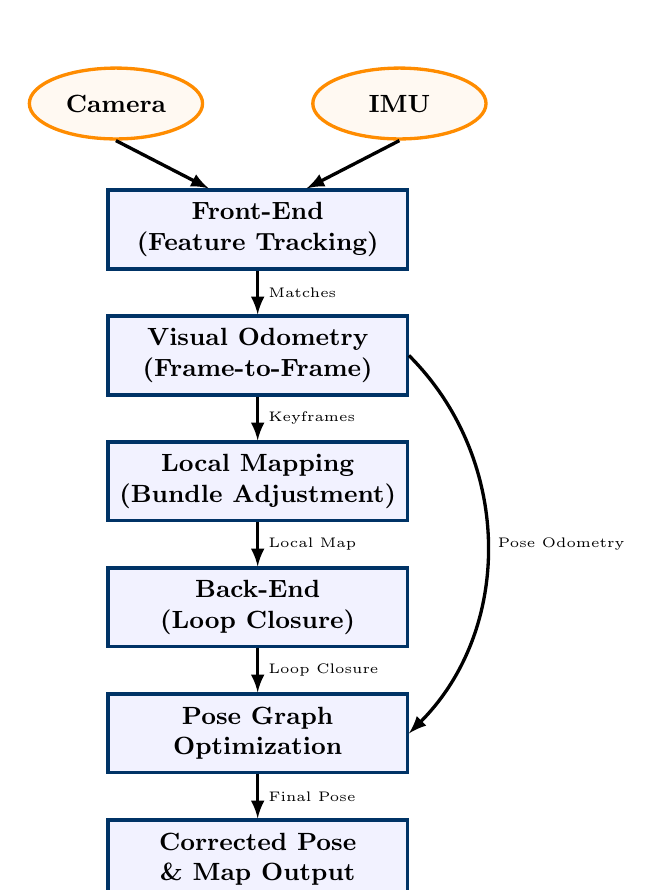
\begin{tikzpicture}[
        node/.style={rectangle, draw=darkblue, very thick, minimum width=3.8cm, minimum height=1.0cm, align=center, fill=blue!5!white, font=\small\bfseries},
        sensor/.style={ellipse, draw=warnorange, very thick, minimum width=2.2cm, minimum height=0.9cm, align=center, fill=orange!5!white, font=\small\bfseries},
        arrow/.style={->, very thick, >=latex, line width=1.2pt}]

        % Nodes
        \node[sensor] (cam) at (0,0) {Camera};
        \node[sensor] (imu) at (3.6,0) {IMU};
        
        \node[node] (fe) at (1.8,-1.6) {Front-End\\(Feature Tracking)};
        \node[node] (vo) at (1.8,-3.2) {Visual Odometry\\(Frame-to-Frame)};
        \node[node] (lm) at (1.8,-4.8) {Local Mapping\\(Bundle Adjustment)};
        \node[node] (lc) at (1.8,-6.4) {Back-End\\(Loop Closure)};
        \node[node] (opt) at (1.8,-8.0) {Pose Graph\\Optimization};
        \node[node] (out) at (1.8,-9.6) {Corrected Pose\\\& Map Output};

        % Connections
        \draw[arrow] (cam.south) -- (fe.140);
        \draw[arrow] (imu.south) -- (fe.40);
        \draw[arrow] (fe.south) -- node[right, font=\tiny]{Matches} (vo.north);
        \draw[arrow] (vo.south) -- node[right, font=\tiny]{Keyframes} (lm.north);
        \draw[arrow] (lm.south) -- node[right, font=\tiny]{Local Map} (lc.north);
        \draw[arrow] (lc.south) -- node[right, font=\tiny]{Loop Closure} (opt.north);
        \draw[arrow] (opt.south) -- node[right, font=\tiny]{Final Pose} (out.north);
        
        % Curved bypass for Visual Odometry Pose update to Pose Graph Optimization
        \draw[arrow, bend left=45] (vo.east) to node[midway, right, font=\tiny]{Pose Odometry} (opt.east);

    \end{tikzpicture}
    \caption{Data Flow and Architecture of the Studied Visual SLAM Pipeline}
\end{figure}

% ============================================================
% 8. CAMERA & SENSOR STUDY
% ============================================================
\section{Camera \& Sensor Study}

\subsection{Camera Types and Acquisition Methods}
Different methods of obtaining camera data were evaluated, including USB-connected cameras and mobile-phone IP camera solutions (streaming over the network). For any onboard, real-time use case, a directly-connected USB or MIPI camera is strongly preferable to a network-streamed source: IP camera links introduce variable latency and compression artifacts, both of which directly degrade feature tracking and pose estimation quality. Network cameras remain useful for quick desk-based experimentation but should not be treated as representative of onboard performance.

Looking ahead to Section \ref{sec:integration}, the camera type chosen materially changes what the SLAM system can do:
\begin{itemize}[noitemsep]
    \item \textbf{Monocular:} A single camera cannot recover absolute scale (it knows shape, not size, unless fused with an IMU or another metric sensor).
    \item \textbf{Stereo:} A stereo pair recovers metric depth directly from the known physical baseline between the two lenses.
    \item \textbf{RGB-D:} A colour camera paired with an active depth sensor (structured light or Time-of-Flight) gives dense depth per pixel but typically has a shorter effective range and can struggle outdoors in bright sunlight.
\end{itemize}

\subsection{Calibration, Distortion, and Synchronization}
Camera calibration, intrinsic parameters, lens distortion, synchronization, and image quality were studied because they directly affect localization and mapping accuracy. Concretely: an uncalibrated or poorly-calibrated camera introduces systematic geometric error into every feature observation, which the SLAM optimizer will faithfully bake into the map and trajectory rather than correct --- calibration errors do not average out, they compound.

Synchronization matters most once an IMU is added: visual-inertial fusion assumes the camera frame and the IMU sample it is paired with were captured at (or very close to) the same instant, and a timestamp offset that seems trivial on the bench can meaningfully hurt fusion accuracy in the air.

% ============================================================
% 9. KNOWLEDGE GAINED
% ============================================================
\section{Knowledge Gained}
The work produced practical, hands-on understanding --- not just conceptual familiarity --- of the following:
\begin{itemize}
    \item \textbf{Texture Dependence:} ORB features and how feature-based tracking degrades on low-texture or repetitive surfaces (a real concern for indoor Search and Rescue [SAR] environments, e.g., bare walls, rubble).
    \item \textbf{Visual Odometry Drift:} Visual odometry and why it accumulates drift over time if left uncorrected by mapping constraints.
    \item \textbf{Map Optimization:} Bundle adjustment and keyframes as the mechanism for keeping local maps accurate without processing every single frame, preserving computational resources.
    \item \textbf{Loop Closure Defense:} Loop closure as the primary defense against long-run drift, and why environments with few revisit opportunities (e.g., a single linear sweep through a collapsed structure) represent the hardest case for SLAM.
    \item \textbf{Map Formats:} Occupancy grids and pose graph optimization as the map representations most directly useful for path planning and obstacle avoidance downstream of SLAM itself.
    \item \textbf{ROS middleware:} ROS-based robotics workflows --- nodes, topics, launch files --- as the integration layer that will carry SLAM output to the flight controller bridge.
    \item \textbf{System Friction:} The practical importance of calibration quality, computational headroom, and sensor quality. These are not academic concerns; they are the difference between a SLAM system that works and one that silently drifts into collision.
\end{itemize}

\newpage

% ============================================================
% 10. PROPOSED INTEGRATION: SLAM ON THE DRONE PLATFORM
% ============================================================
\section{Proposed Integration: SLAM on the Drone Platform}
\label{sec:integration}
This section moves beyond the original report's scope to lay out a concrete path from the current research foundation to an onboard, flight-tested capability, integrated with our existing ArduPilot-based airframes and AERO-GCS.

\subsection{Hardware Architecture}
SLAM at useful frame rates needs dedicated onboard compute --- it cannot run on the flight controller itself. The recommended architecture is a companion computer, connected to the flight controller over a serial or USB link running MAVLink, mirroring the ground-side architecture already used for the SAR detection pipeline.
\begin{itemize}
    \item \textbf{Companion computer:} An NVIDIA Jetson-class board (e.g., Orin Nano / Orin NX) is the natural choice --- it has the GPU headroom to run RTAB-Map and, notably, could share compute with the existing YOLOv8 SAR detection model if both are ever needed on the same mission, since both are already CUDA-accelerated workloads in our stack.
    \item \textbf{Camera:} A stereo or RGB-D module with a built-in IMU (e.g., an Intel RealSense--class depth camera) is preferable to a plain monocular USB webcam --- it removes the scale-ambiguity problem and gives RTAB-Map a metric depth source directly, rather than relying solely on visual-inertial fusion for scale.
    \item \textbf{IMU:} The flight controller's own IMU can supplement or cross-check the camera-integrated IMU, but for tight time synchronization, the camera's own IMU is generally the one fed directly into the SLAM node.
    \item \textbf{SWaP Budget:} This is an additive payload on top of the existing SAR/GCS hardware envelope (Skydroid H12 link, RTSP camera, etc.) and needs to be budgeted explicitly against current AUW and flight-time figures rather than assumed to be free.
\end{itemize}

\subsection{Software Stack \& Data Flow}
The proposed software chain runs entirely on the companion computer, with only a thin telemetry bridge crossing to the flight controller:
\begin{enumerate}
    \item Camera + IMU driver publishes synchronized image and inertial data as ROS 2 topics.
    \item An \texttt{rtabmap\_ros} node consumes those topics and publishes real-time odometry (\texttt{nav\_msgs/Odometry}) plus, as compute allows, an occupancy grid and/or point cloud.
    \item A MAVROS bridge node converts that ROS 2 odometry into the corresponding MAVLink message (\texttt{VISION\_POSITION\_ESTIMATE} or \texttt{ODOMETRY}) and sends it to the flight controller over the existing serial/USB telemetry link.
    \item ArduPilot's EKF3 is configured (via its \texttt{EK3\_SRC} source-selection parameters) to accept this external vision source as a position/velocity input, either replacing GPS entirely in fully GPS-denied flight or running alongside it for cross-checking.
\end{enumerate}

\subsection{Integration with ArduPilot / MAVLink}
This is the step that turns ``SLAM running on a bench'' into ``SLAM the autopilot actually trusts.'' ArduPilot's EKF is already designed to fuse an external navigation source through the \texttt{VISION\_POSITION\_ESTIMATE} / \texttt{ODOMETRY} message pair. The main engineering work on our side is:
\begin{enumerate}[label=(\alph*)]
    \item Getting the MAVROS bridge configured and timestamp-aligned correctly.
    \item Tuning \texttt{EK3\_SRC} and the associated noise parameters so the EKF weights vision input appropriately relative to other sensors.
    \item Validating behaviour in ArduPilot's SITL simulator before any hardware-in-the-loop test, exactly as AERO-GCS development already does for other features.
\end{enumerate}

\subsection{Integration with AERO-GCS}
Since AERO-GCS is our own Mission Planner--derived ground station, it is well positioned to become the operator-facing window into this system rather than treating SLAM as an invisible background process. Concretely:
\begin{itemize}
    \item \textbf{Live Map Panel:} Showing the SLAM-generated occupancy grid or point cloud as it builds during flight --- directly useful for a SAR operator trying to understand the interior of a structure in real time.
    \item \textbf{Status Indicator:} A navigation-source status indicator (GPS / Vision / Fused), so the operator always knows what the EKF is currently trusting --- critical for safety awareness during a GPS-to-vision handover.
    \item \textbf{SAR Overlay:} Optionally, overlaying SAR detection results (from the existing YOLOv8 pipeline) onto the SLAM-built map, so a detection made indoors can be shown at its actual position within the structure.
\end{itemize}

\subsection{Phased Implementation Plan}
The path forward is structured into seven distinct phases to manage risk:

\begin{table}[H]
    \centering
    \small
    \renewcommand{\arraystretch}{1.3}
    \begin{tabularx}{\textwidth}{@{}l p{4.2cm} p{6.8cm} l@{}}
        \toprule
        \textbf{Phase} & \textbf{Milestone} & \textbf{Activities} & \textbf{Status} \\
        \midrule
        \textbf{0} & Research foundation & Framework evaluation, environment setup, pipeline understanding & Complete \\
        \midrule
        \textbf{1} & Bench validation & Static camera + companion computer rig; validate RTAB-Map mapping accuracy & Next \\
        \midrule
        \textbf{2} & Handheld / walked test & Carry the rig through an indoor space; evaluate drift, loop closure, and map quality & Planned \\
        \midrule
        \textbf{3} & SITL telemetry bridge & MAVROS + \texttt{EK3\_SRC} configuration validated against ArduPilot SITL simulator & Planned \\
        \midrule
        \textbf{4} & Grounded hardware-in-loop & Full rig mounted on the airframe, propellers off; validate real telemetry flow end-to-end & Planned \\
        \midrule
        \textbf{5} & Caged/indoor GPS-denied hover & Controlled indoor flight test (netted area) validating vision-based position hold & Planned \\
        \midrule
        \textbf{6} & Field / SAR-relevant test & Structured test in a building- or tunnel-like environment representative of SAR use & Future \\
        \bottomrule
    \end{tabularx}
    \caption{Phased Integration and Flight Testing Plan}
\end{table}

\subsection{Use Case: SAR / GPS-Denied Operations}
This work directly complements the existing SAR detection system: today, that system's detections are only as useful as the GPS/telemetry position attached to them, which is exactly what is unavailable in the environments SAR most needs --- collapsed structures, tunnels, dense interiors. A working SLAM stack would let the drone build and share a local map of such a space even with no GPS at all, and would let detections be placed within that map rather than left as an unplaced video frame. That combination --- local mapping plus geo-referenced detection --- is a legacy-free improvement.

\subsection{Safety \& Failover Considerations}
\begin{itemize}
    \item \textbf{Graceful Degradation:} SLAM-based position must degrade gracefully, not silently --- a lost-tracking event should trigger an explicit failsafe behaviour (e.g., hold last known position and alert), not an unnoticed drift into bad state.
    \item \textbf{Lane Switching:} Where GPS is intermittently available, GPS and vision estimates should be cross-checked rather than blindly switched between, using ArduPilot's EKF lane-switching behaviour as the underlying mechanism.
    \item \textbf{Feature-Poor Environments:} Feature-poor environments (bare walls, smoke, low light) are the realistic failure mode for feature-based SLAM and should be treated as an expected condition to test for, not an edge case.
    \item \textbf{Conservative Guidance:} Any autonomous behaviour commanded from a vision-derived position estimate should be more conservative (lower speed/acceleration limits) than the same behaviour under a trusted GPS fix, at least until the vision pipeline has a flight-proven track record.
\end{itemize}

% ============================================================
% 11. RISKS & CHALLENGES
% ============================================================
\section{Risks \& Challenges}
\begin{itemize}
    \item \textbf{Computational Load:} RTAB-Map competing with other onboard workloads (e.g., YOLOv8 SAR inference) for the same companion computer's GPU/CPU budget needs explicit profiling, not an assumption that both fit comfortably.
    \item \textbf{Vibration \& Motion Blur:} A multirotor's vibration environment is harsher than the bench/handheld testing done so far and can meaningfully degrade feature tracking; mechanical isolation for the camera mount is likely necessary.
    \item \textbf{Lighting \& Texture Dependence:} Feature-based SLAM struggles in low light and on low-texture surfaces --- a real concern for indoor SAR scenes.
    \item \textbf{SWaP Budget:} Size, weight, and power limits represent a hard constraint. Adding companion hardware and active sensors directly impacts the battery endurance model.
    \item \textbf{Integration Complexity:} Bridging a research-grade SLAM stack into a certified-feeling, safety-relevant flight-control input is a materially bigger engineering lift than getting the same stack running for visualization on a bench.
\end{itemize}

% ============================================================
% 12. FUTURE SCOPE
% ============================================================
\section{Future Scope}
\begin{itemize}
    \item \textbf{MAVLink Bridging:} Integrate RTAB-Map with ArduPilot via the MAVROS bridge described in Sections \ref{sec:integration}.2 and \ref{sec:integration}.3.
    \item \textbf{Real-Time 3D Mapping:} Generate real-time 3D maps usable both onboard (for obstacle avoidance) and on the ground (for operator situational awareness).
    \item \textbf{Sensor Fusion Optimization:} Combine SLAM output with existing telemetry (barometric altitude, optical flow) for a single, fused navigation picture.
    \item \textbf{Obstacle Avoidance:} Implement autonomous obstacle avoidance using the occupancy grid / point cloud output as an input to path planning.
    \item \textbf{AI Pipeline Integration:} Integrate the existing AI-based (YOLOv8) object/person detection pipeline with SLAM-derived positioning, so SAR detections are placed within the built map.
    \item \textbf{GCS Visualization:} Visualize localization data --- pose, map, navigation-source status --- natively within AERO-GCS.
\end{itemize}

% ============================================================
% 13. CONCLUSION
% ============================================================
\section{Conclusion}
This research established a solid technical foundation in SLAM concepts, Linux robotics development, ROS 2 integration, and the beginnings of autonomous navigation work relevant to our platform. It was, by design, a research and environment-preparation phase rather than a deployed system --- and that sequencing was the right call, since the framework, hardware, and integration decisions made here directly shape whether the eventual onboard implementation is a straightforward bring-up or a difficult retrofit. Section \ref{sec:integration} of this report turns that research into an actionable, phased plan for getting SLAM from a bench evaluation into a flight-tested, GPS-denied navigation capability integrated with our existing ArduPilot airframes and AERO-GCS.

% ============================================================
% 14. REFERENCES & FURTHER READING
% ============================================================
\section{References \& Further Reading}
\begin{itemize}
    \item Campos, C. et al. --- ``ORB-SLAM3: An Accurate Open-Source Library for Visual, Visual-Inertial and Multi-Map SLAM'' (IEEE Transactions on Robotics).
    \item Labbé, M. \& Michaud, F. --- ``RTAB-Map as an Open-Source Lidar and Visual SLAM Library for Large-Scale and Long-Term Online Operation'' (Journal of Field Robotics).
    \item ROS 2 (Jazzy Jalisco) official documentation --- \url{docs.ros.org}.
    \item ArduPilot documentation --- EKF3 external navigation / non-GPS navigation sources --- \url{ardupilot.org}.
    \item RTAB-Map project documentation and ROS 2 integration guide --- \url{introlab.github.io/rtabmap}.
\end{itemize}

\end{document}
